% VentureTruth Research Poster - A0 Portrait - Single Column Design
\documentclass[25pt, a0paper, portrait]{tikzposter}

% ==================== PACKAGES ====================
\usepackage[utf8]{inputenc}
\usepackage{graphicx}
\usepackage{amsmath}
\usepackage{amssymb}
\usepackage{xcolor}
\usepackage{fontawesome5} % Requires XeLaTeX or LuaLaTeX recommended
\usepackage{enumitem}
\usepackage{booktabs}
\usepackage{tcolorbox}
\usepackage{lmodern}
\usepackage{array}
\usepackage{changepage}
\usepackage{subcaption}

% ==================== TIKZ SETUP ====================
\usetikzlibrary{shapes.geometric, arrows.meta, positioning, calc, shadows.blur}

% ==================== THEME & COLORS ====================
\usetheme{Simple}

% Custom Colors
\definecolor{primary}{RGB}{0, 70, 120}       % Deep Blue
\definecolor{accent}{RGB}{210, 65, 55}       % Crimson Red
\definecolor{success}{RGB}{45, 125, 90}      % Forest Green
\definecolor{warning}{RGB}{200, 140, 40}     % Amber
\definecolor{neutral}{RGB}{90, 90, 100}      % Slate Gray
\definecolor{lightbg}{RGB}{248, 248, 252}    % Light Gray Blue

% Block Style
\defineblockstyle{Scientific}{
    titlewidthscale=1, bodywidthscale=1, titlecenter,
    titleinnersep=15pt, bodyinnersep=20pt,
    titleoffsetx=0pt, titleoffsety=0pt, bodyoffsetx=0pt, bodyoffsety=0pt
}{
    \draw[color=blocktitlebgcolor, fill=blocktitlebgcolor!5, line width=3pt, rounded corners=10pt]
        (blocktitle.south west) rectangle (blocktitle.north east);
    \draw[color=white, line width=0pt] (blockbody.south west) rectangle (blockbody.north east); % Invisible body border
}
\useblockstyle{Scientific}

% Global Color Assignments
\colorlet{blocktitlebgcolor}{primary}
\colorlet{blocktitlefgcolor}{black}
\colorlet{blockbodybgcolor}{white}
\colorlet{blockbodyfgcolor}{black}

% ==================== METADATA ====================
\title{\parbox{\linewidth}{\centering \Huge \textbf{VentureTruth}: Automated Verification of Startup Pitch Claims\\ \Large}}
\author{\textbf{Yufei Yang, 
Mykhailo Riabets \& Zekai Li}}
\institute{\faUniversity\ Technical University of Munich \quad | \quad \faLaptopCode\ Natural Language Processing Lab}

% ==================== DOCUMENT START ====================
\begin{document}

\maketitle[width=0.98\linewidth, titletotopverticalspace=0.9cm]

% ==================== SINGLE COLUMN START ====================

% -------------------- RESEARCH CONTEXT --------------------

\begin{columns}
    \column{0.5}
    \block{1. Context: Startup pitch decks are high-volume, self-promotional documents}{
      
    
        \vspace{0.6em}
        \begin{itemize}[itemsep=0.6em, leftmargin=1.2em]
            \item Venture Capital investors on average screen \textbf{thousands} of pitch decks per year
            \item These pitch decks contain claims that mix facts, internal metrics, and promotional language.
            \item Screening these documents can be inefficient and requires analysts to do verification of startup claims manually
        \end{itemize}
    
        \vspace{0.4em}
        \textit{\textcolor{neutral}{→ Persistent information asymmetry between founders and investors.}}
    }
    \column{0.5}
    \block{2. Research Problem: How effectively can LLMs verify startup claims?}{
        \textbf{\textcolor{primary}{Core Approach}}
       The contributions of this work include:

        \begin{itemize}
            \item The contributions of this work include:
We evaluate the ability of large language models to extract and verify structured metadata from heterogeneous startup artifacts.
            \item We study the effectiveness of large language models for identifying, extracting, and verifying claims, with a focus on multi-source, iterative verification.
            \item We propose a novel end-to-end architecture for processing startup pitch decks that integrates claim extraction, evidence retrieval, iterative verification, and robustness auditing.
        \end{itemize}
    }
\end{columns}

% -------------------- METHODOLOGY --------------------
\block{3. Solution: LLM-Based Claim Verification Pipeline for VC Due Diligence}{
  \centering
  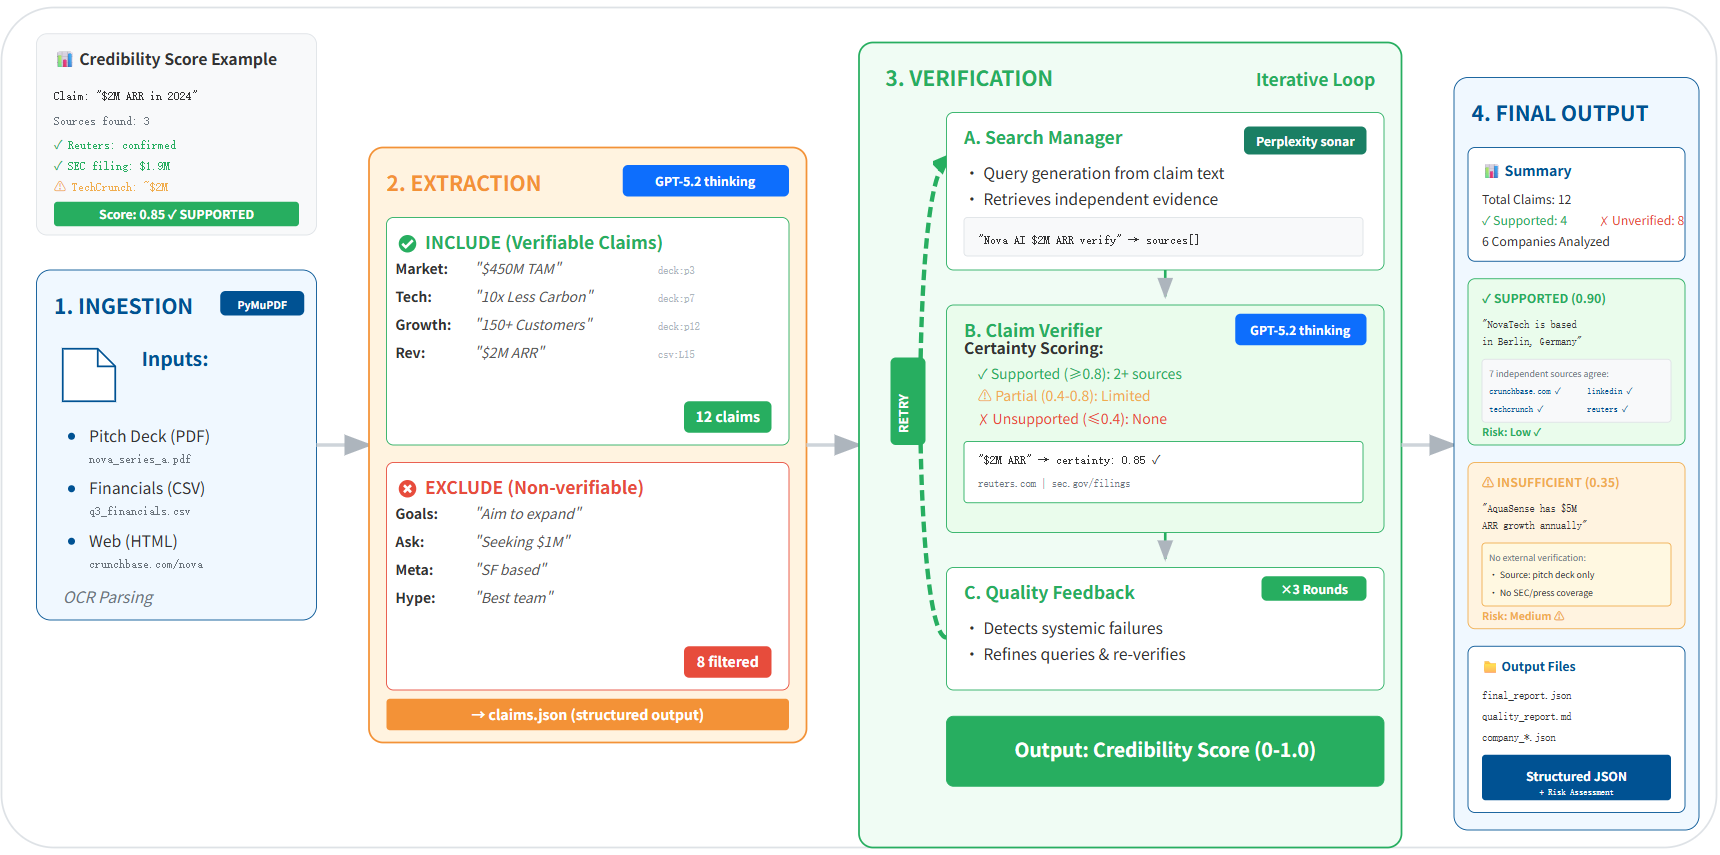
\includegraphics[width=\linewidth]{pipeline v2.png}

  \vspace{-0.3em}

  An end-to-end NLP pipeline for extracting and verifying factual claims from startup pitch decks.

  \begin{tcolorbox}[
    colback=primary!10,
    colframe=primary,
    title=Key Innovations,
    fonttitle=\bfseries,
    top=2mm,
    bottom=2mm,
    boxsep=2mm
  ]
  \begin{itemize}[topsep=2pt, itemsep=2pt, leftmargin=*]
    \item \textbf{Novel application of Large Language Models (LLMs)} to systematically verify self-promotional claims in startup pitch materials.
    \item \textbf{Evaluation of LLMs as claim verification tools}, assessing classification into \emph{Supported}, \emph{Contradicted}, or \emph{Insufficient Evidence}.
    \item \textbf{Verification with explanations}: Natural language explanations support for calibrating investor decision-making, such as downstream screening.
  \end{itemize}
  \end{tcolorbox}
}


% -------------------- RESULTS --------------------







% Start the columns environment to put Block 4 and 5 side-by-side
\begin{columns}
    % --- COLUMN 1 (Block 4) ---
    \column{0.7} 
    \block{4. Evaluation of Results}{
        
        % --- Image 1 (Left) ---
        \begin{minipage}{0.3\textwidth}
            \centering
            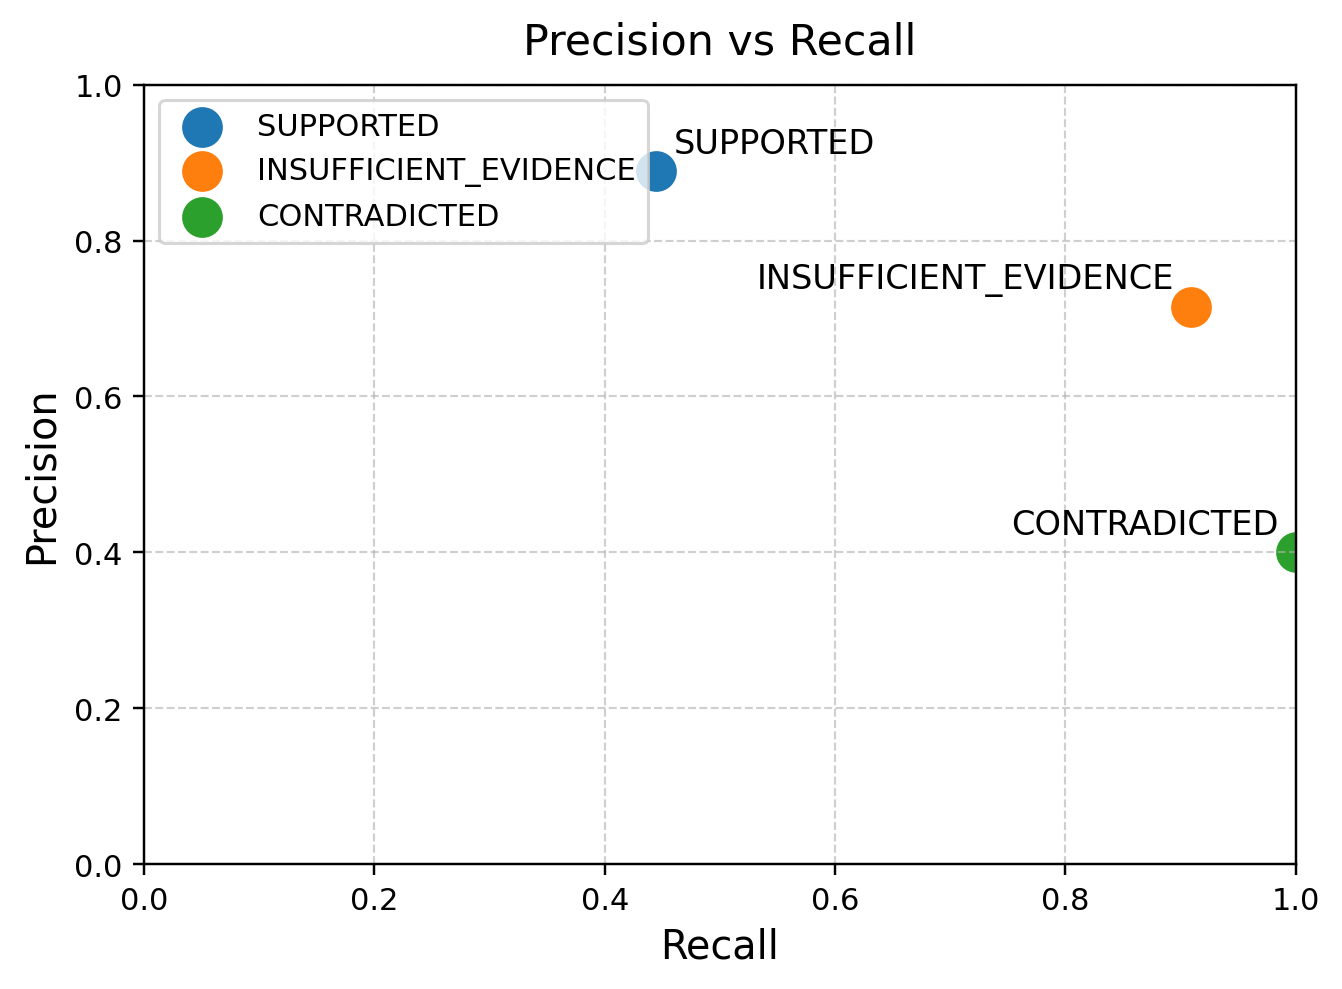
\includegraphics[width=\textwidth]{poster_diagrams/per_class_points_precision_vs_recall.png}
            
            % --- Caption 1 ---
            \par \vspace{0.5em} \small \textit{
                Figure 1: The Supported class achieves high precision, whereas the Contradicted class prioritizes recall.
            }
        \end{minipage}
        \hspace{0.5cm} % Gap
        % --- Image 2 (Right) ---
        \begin{minipage}{0.35\textwidth}
            \centering
            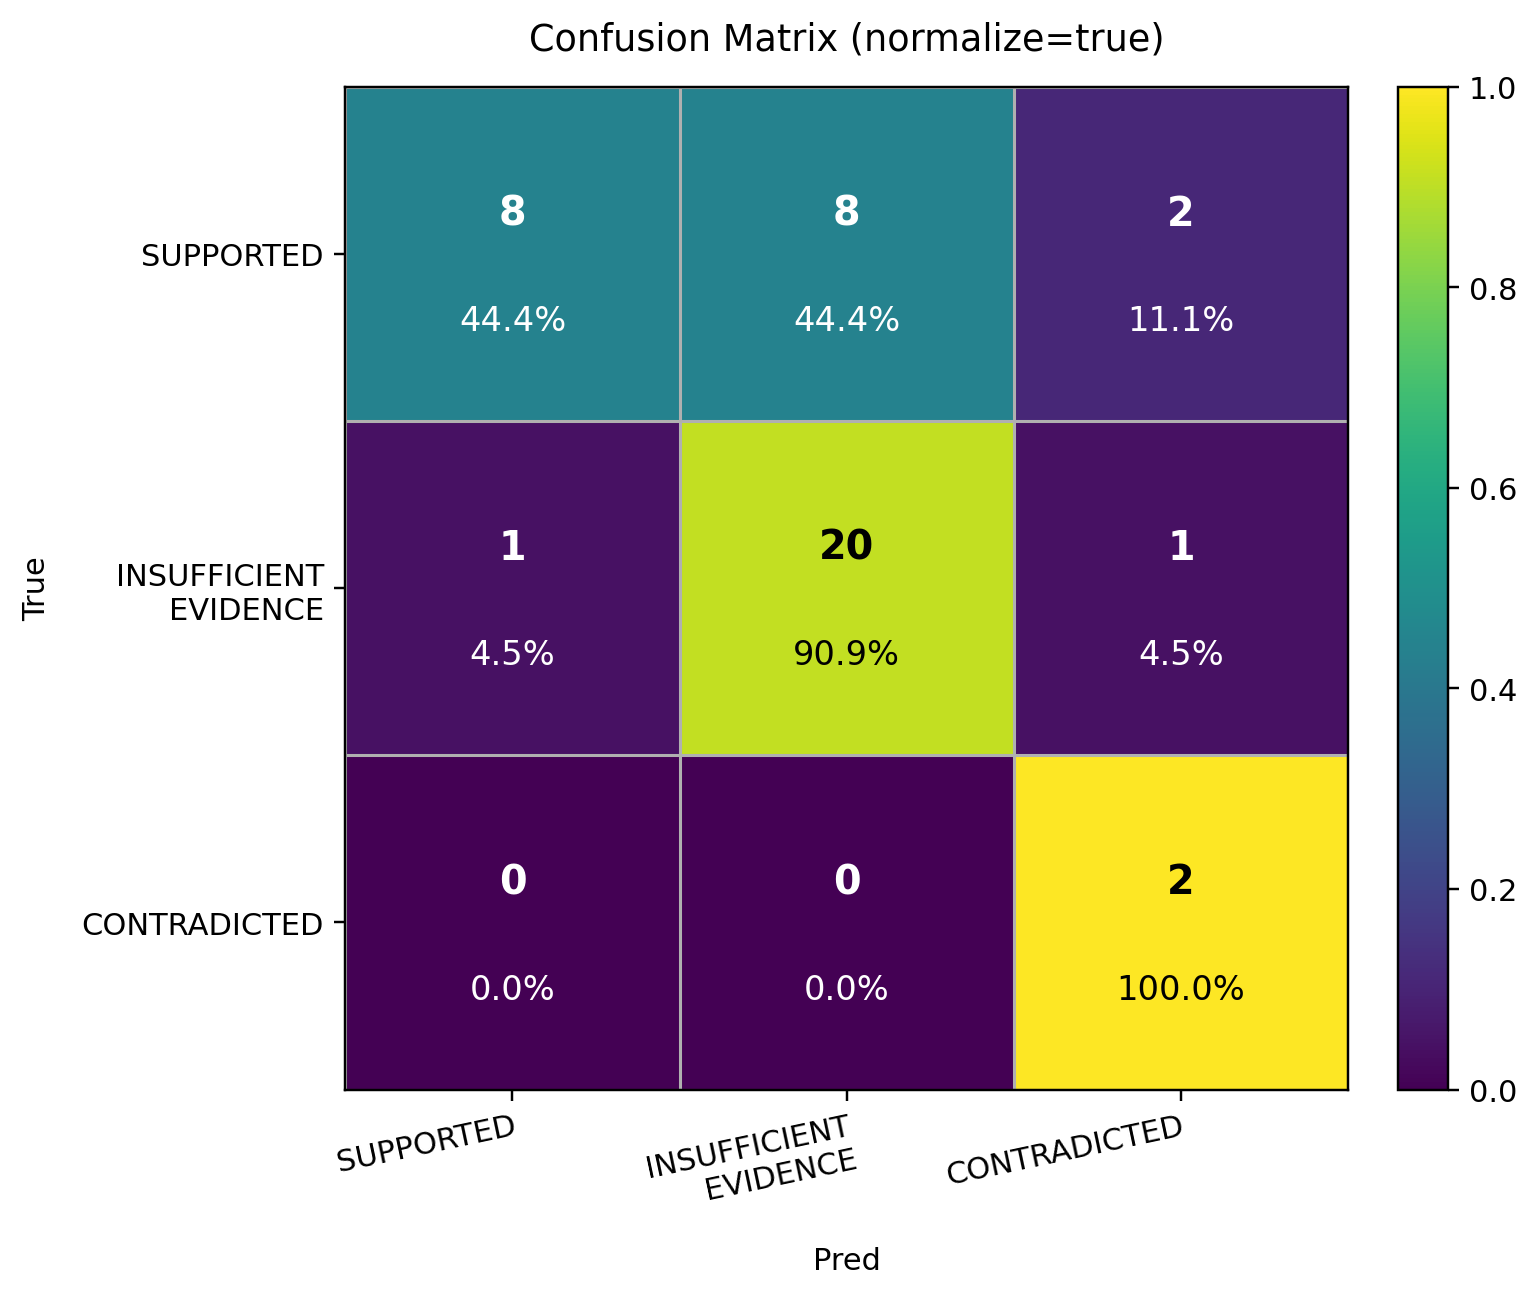
\includegraphics[width=\textwidth]{poster_diagrams/cm3x3_norm_true.png}
            
            % --- Caption 2 (New) ---
            \par \vspace{0.5em} \small \textit{
                Figure 2: High accuracy is observed for Insufficient Evidence (90.9\%) and Contradicted (100\%) classes.
            }
        \end{minipage}
        
        \vspace{1em}
        \label{fig:results}
    }

    
% % -------------------- IMPACT --------------------


    % --- COLUMN 2 (Block 5) ---
    \column{0.3} % Remaining 50%
    \block{5. Impact \& Future Directions}{
        \begin{tcolorbox}[colback=primary!5, colframe=primary, title=\textbf{Why It Matters}, fonttitle=\bfseries]
            % Internal columns for the tcolorbox
           \begin{columns}
  \column{0.5}
  \begin{minipage}{\linewidth}
    \centering
    \textcolor{primary}{\faChartLine}\\
    \textbf{For Investors}\\
    DD time: Weeks $\to$ Hours
  \end{minipage}

  \column{0.5}
  \begin{minipage}{\linewidth}
    \centering
    \textcolor{warning}{\faMicroscope}\\
    \textbf{For Research}\\
    Cornerstone LLM-Based Startup Claim Verification
  \end{minipage}
\end{columns}

        \end{tcolorbox}

        \vspace{1.5em}
        \textbf{Future Work Directions:}
        \begin{enumerate}[label=\textbf{\arabic*.}, itemsep=0.8em, leftmargin=1.5em]
            \item \textbf{Workflow Customization:} Allow model selection for each individual step.
            \item \textbf{Dataset Expansion:} Increase sample sizes for more robust evaluation.
            \item \textbf{Broader LLM Benchmarking:}Test additional models, including open-source LLMs.
            \item \textbf{Multimodal Integration:} Extend extraction to video and audio formats.
        \end{enumerate}
    }
\end{columns}

% % -------------------- CONTACT --------------------
% \block{Resources}{
%     \centering
%     \begin{minipage}{0.7\linewidth}
%         \centering

%         % NOTE: Some tikzposter setups do not define `tikzfigure`.
%         % Use plain tikzpicture for maximum compatibility.
%         \begin{tikzpicture}
%             \draw[fill=white] (0,0) rectangle (4,4);
%             \node at (2,2) {\Huge \faQrcode};
%             \node[below] at (2,0) {\textbf{Scan for Demo}};
%         \end{tikzpicture}

%         \vspace{1em}
%         \Large
%         \faGithub\ \texttt{github.com/venturetruth} \quad
%         \faEnvelope\ \texttt{venturetruth@tum.de}
%     \end{minipage}
% }

% ==================== SINGLE COLUMN END ====================




% ==================== 底部左下角图片 ====================
   \node[anchor=south west, inner sep=0pt, xshift=2cm, yshift=2cm] at (bottomleft) {
    % 将 width=4cm 改为你想要的大小 (例如 3cm, 5cm)
    
\includegraphics[width=3cm]{GithubRepoQR.png} 
};



\end{document}
